\title{Modular Deep Encoder-Decoders}
\author{Sebastian Arnold\Mark{1}, Prashanth Gurunath Shivakumar\Mark{2}, Cheng Qu\Mark{3}\\ and Qiangui Huang\Mark{4}}
%\affil[1]{Department of Computer Science, University of Southern California, Los Angeles, CA \authorcr Email: {\tt \{arnolds, chengqu, qianguih\}@usc.edu}\vspace{1.5ex}}
%\affil[2]{Ming Hsieh Department of Electrical Engineering, University of Southern California, Los Angeles, CA \authorcr Email: {\tt pgurunat@usc.edu} \vspace{-2ex}} 

\documentclass[12pt]{article}
\usepackage{amsfonts}
% Packages import
\usepackage[utf8]{inputenc}
\usepackage[T1]{fontenc}
\usepackage[english]{babel}
\usepackage{fancyhdr}
\usepackage{amsthm}
\usepackage{amsmath}
\usepackage{amssymb}
\usepackage{xpatch}
\usepackage{titling}
\usepackage{geometry}
\usepackage{multicol}
\usepackage{lipsum}
\usepackage{array}
\usepackage{algorithm}
\usepackage{algorithmicx}
\usepackage[noend]{algpseudocode}
\usepackage{listing}
\usepackage{graphicx}
\usepackage{longtable}
\usepackage{supertabular}
\usepackage{booktabs}
\usepackage{float}
\usepackage{hyperref}
\usepackage[export]{adjustbox}
\usepackage{breakcites}
\usepackage{color}
\usepackage{fancyvrb}
\usepackage{listings}
\usepackage{xcolor}

% Defining variables
\makeatletter
\let\Title\@title
\let\Author\@author
\let\Date\@date
\makeatother

% Margins
%\geometry{letterpaper, portrait, margin=1.00in}
%\geometry{legalpaper, portrait, margin=1.00in}
\geometry{a4paper, portrait, margin=1.00in, bottom=1.25in, top=1.25in}
 
% Headers and Footers
\pagestyle{fancy}
\fancyhf{}
\rhead{\Title}
\lhead{\Date}
\rfoot{Page \thepage}
\renewcommand{\headrulewidth}{2pt}
\renewcommand{\footrulewidth}{1pt}
\renewcommand{\qedsymbol}{$\blacksquare$}

% Section Customization
\renewcommand\thesection{{\Roman{section}}}
\renewcommand\thesubsection{}{\Roman{subsection}}
\renewcommand\thesubsubsection{}{\Roman{subsubsection}}

% Theorems and Tipps
\makeatletter
\xpatchcmd{\@thm}{\thm@headpunct{.}}{\thm@headpunct{}}{}{}
\newtheorem{theorem}{\underline{Theorem}}[section]
\newtheorem{definition}{\underline{Definition}}[section]
\newtheorem{corollary}{Corollary}[theorem]
\newtheorem{lemma}[theorem]{Lemma}
\theoremstyle{remark}
\newtheorem*{note}{Note:}
\theoremstyle{remark}
\newtheorem*{tip}{Tip:}

% Limit Image Width
\let\oldincludegraphics\includegraphics
\renewcommand{\includegraphics}[2][]{%
  \oldincludegraphics[#1,max width=\linewidth]{#2}}

% Code highlighting
\newcommand{\VerbBar}{|}
\newcommand{\VERB}{\Verb[commandchars=\\\{\}]}
\DefineVerbatimEnvironment{Highlighting}{Verbatim}{commandchars=\\\{\}}
\newenvironment{Shaded}{}{}
\newcommand{\KeywordTok}[1]{\textcolor[rgb]{0.00,0.00,1.00}{{#1}}}
\newcommand{\DataTypeTok}[1]{{#1}}
\newcommand{\DecValTok}[1]{{#1}}
\newcommand{\BaseNTok}[1]{{#1}}
\newcommand{\FloatTok}[1]{{#1}}
\newcommand{\CharTok}[1]{\textcolor[rgb]{0.00,0.50,0.50}{{#1}}}
\newcommand{\StringTok}[1]{\textcolor[rgb]{0.00,0.50,0.50}{{#1}}}
\newcommand{\CommentTok}[1]{\textcolor[rgb]{0.00,0.50,0.00}{{#1}}}
\newcommand{\OtherTok}[1]{\textcolor[rgb]{1.00,0.25,0.00}{{#1}}}
\newcommand{\AlertTok}[1]{\textcolor[rgb]{1.00,0.00,0.00}{{#1}}}
\newcommand{\FunctionTok}[1]{{#1}}
\newcommand{\RegionMarkerTok}[1]{{#1}}
\newcommand{\ErrorTok}[1]{\textbf{{#1}}}
\newcommand{\NormalTok}[1]{{#1}}
\lstnewenvironment{code}{\lstset{language=Haskell,basicstyle=\small\ttfamily}}{}


\newcommand\Mark[1]{\textsuperscript#1}

% Custom Title
\def\maketitle{
	\par\rule{\textwidth}{2pt}
	\par\hfill
	\begin{centering}
	\begingroup
	\centering
	{\par\textbf{\LARGE\@title}\\[1.5em]
	\large\par{\textit{\@author}}}\\[1em]
	\begin{tabular}{*{4}{>{\centering}p{.23\textwidth}}}
	\url{arnolds@usc.edu}\Mark{1} & \url{pgurunat@usc.edu}\Mark{2} & \url{chengqu@usc.edu}\Mark{3} & \url{qianguih@usc.edu}\Mark{4} \tabularnewline
	9013085897 & 2251924199 & 9532576000 & 2385279985
	\end{tabular}\par
	\endgroup
	\par\rule{\textwidth}{2pt}
	\end{centering}
}

\begin{document}
\thispagestyle{empty}
\maketitle
\hfill
\begin{abstract}
%In this short paper we propose an approach to transfer learning using rich
%vector embeddings. The suggested technique can be applied to any supervised
%task, and it handles multiple sources and changing sources of data without the
%need for retraining. To verify our ideas, we apply our ideas to the task of
%text-classification.

In this short paper, we propose a Modular Deep Encoder-Decoder network (MDED) for text classification. The basic idea behind MDED is to extend a pre-trained model, which consists of a set of deep encoder-decoders, with an additional source of data modality by adding a new encoder to the network. MDED has been applied to text classification on SaudiNewsNet. A modular Long Short Term Memory (LSTM) network is built. Experimental results show that our algorithm can efficiently combine new source of data and pre-trained model. (show some summaries of experimental results here)

\end{abstract}

\section{Introduction}\label{introduction}

%Our goal is to generate rich vector embeddings from articles to classify
%them into predefined categories. Then, we want to extend our model with
%an additional source of data: the title of the videos. To handle this
%new knowledge source without retraining our previous model, we suggest
%to generate a new embedding that will be used to modify the original
%one. This combined embedding will then be used for the classification
%task.

In the past decade, deep learning has gained a lot of momentum in various fields. It has been successfully applied to natural language processing (NLP). End-to-end trained deep learning algorithms have been proven to outperform traditional algorithms on various NLP tasks. The success of deep learning is accounted for trading off computationally complexity for performance. The high complexity demand for training deep learning algorithms is inefficient especially when there is new complementary data modality to be used to update a model and re-train it from scratch every time. To alleviate this problem, a novel Modular Deep Encoder-Decoder network (MDED) is proposed in this paper. The basic idea behind MDED is to extend a pre-trained model, which consists of a set of deep encoder-decoders, with an additional source of data modality by adding a new encoder to the network. 


More formally, we want to jointly learn a set of \emph{encoder}
functions $\{E_i\}_0^N$ mapping samples $x \sim \chi_i$ from a set of
data distributions $\{\chi_i\}_0^N$ to a fixed-sized vector embedding
$V$.

\[ \forall i \in [0; N]: E_i(x): \chi_i \rightarrow V_i \in \Re^M\]

\[V = \sum_i^N V_i\]

The embedding $V$ is then fed into a decoder function $D$ which in the
case of classification learns a mapping from the vector space of $V$ to
the label space $L$.

\[ D(v): \Re^M \rightarrow L \in \Re^D\]

Finally, we want to extend the set of encoders by learning a new encoder
$E_{N+1}$ which handles samples from a different dataset $\chi_{N+1}$,
without retraining our trained decoders and encoders.

\[ E_{N+1}(x): \chi_{N+1} \rightarrow V_{N+1} \in \Re^M\]

\begin{figure}[htbp]
\centering
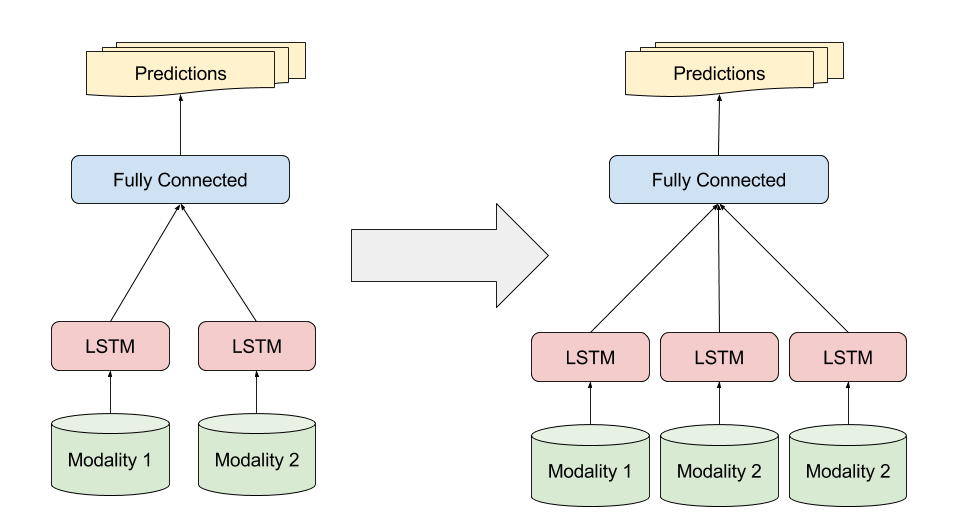
\includegraphics{figures/multimodal.png}
\caption{Multi-modal Transfer Learning}
\end{figure}

Although we could have used any kind of mapping, we chose to use deep
learning algorithms, as they easily learn hierarchical representations
and have been known to highly outperform other statistical techniques on
natural language tasks. Learning embeddings has been previously done by
\cite{zhuang2015supervised}, although our proposed contribution is
slightly different. \cite{zhuang2015supervised} used deep autoencoders to
obtain a better initialization of the parameters of their model. Our
approach instead is much closer in spirit to the work of Sutskever
\cite{sutskever2014sequence} and Vinyals \cite{vinyals2015grammar}. They
both use encoders on a sequence of data to generate a
\emph{thought-vector} which will then be decoded in the desired target
sequence. In some sense, our proposal adds the transfer learning
component to their contribution. This approach is also similar to the
work of Karpathy \& al \cite{karpathy2014deep} where they mapped
images to their captions with embeddings.

In this paper, we evaluate the effectiveness of idea by applying the concept towards a simple NLP classification task. We adopt an Arabic newspaper article database to classify into different journals based on the article content, author and title.

\section{Method}\label{method}
\subsection{Materials}
We used the freely available dataset from
\url{https://github.com/ParallelMazen/SaudiNewsNet} The dataset contains
a total of 31,030 Arabic newspaper articles, with a total number of 8,758,976 words. 

\begin{figure}[h!]
\centering
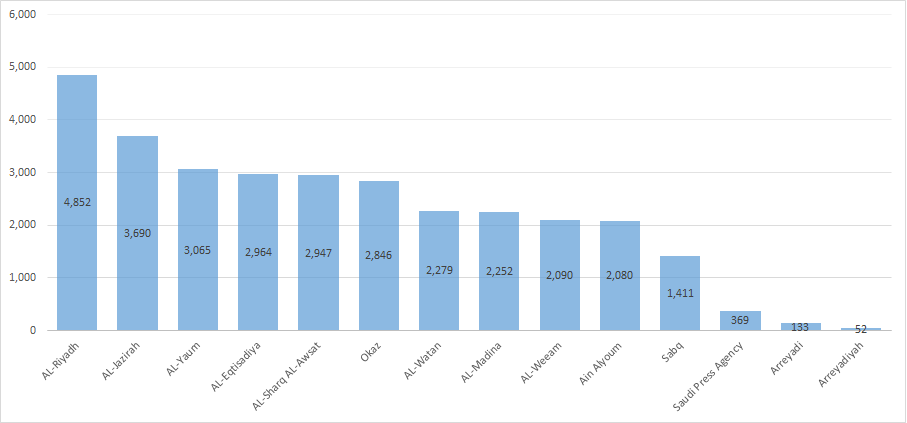
\includegraphics[width=\textwidth]{figures/article-newspaper_distribution.png}
\caption{Figure shows article-newspaper distribution}
\end{figure}

Article objects are represented in json format, with UTF-8 encoding. We wrote a script to download the data from github repo, unzip each file, and read them in as json objects. Each json object contains the following fields:

\begin{itemize}
\item source: A string identifier of the newspaper from which the article was extracted.
\item url: The full URL from which the article was extracted.
\item date\_extracted: The timestamp of the date on which the article was extracted. It has the format YYYY-MM-DD hh:mm:ss. 
\item title: The title of the article. 
\item author: The author of the article.
\item content: The content of the article.
\end{itemize}

The dataset is partitioned into training, development and testing subsets. 80\% of the data is assigned for training and 10\% for development and testing. The development set is utilized for hyper-parameter tuning and the results are finally presented on the testing set. During partitioning, care is taken to ensure appropriate percentage of data is seen in all the classes. Figure~\ref{fig:dist} shows the distribution of data used for training and testing in each class. Figure~\ref{fig:sent_dist} shows the distribution of sentence lengths of the content of the articles.

\begin{figure}[h!]
\centering
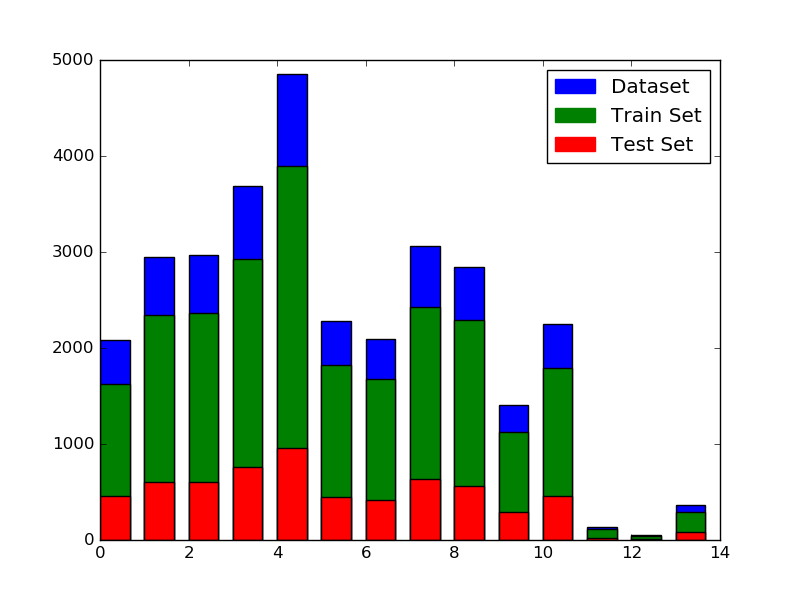
\includegraphics[width=\textwidth]{figures/test_class_distribution.png}
\caption{Distribution of data for training and testing}\label{fig:dist}
\end{figure}

\begin{figure}[t]
\centering
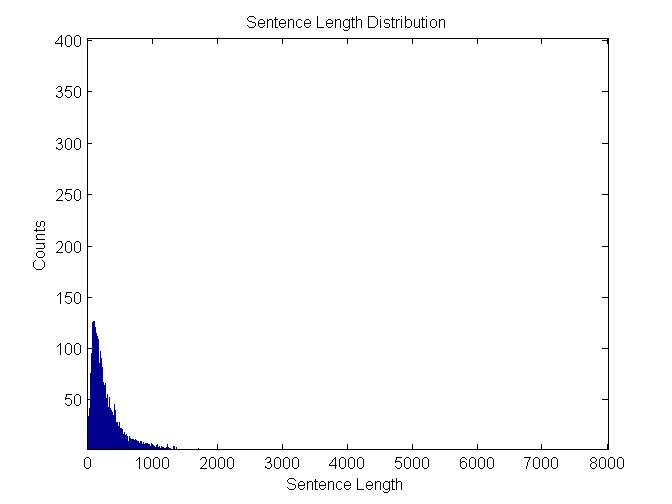
\includegraphics[width=\textwidth,height=6cm]{figures/sentence_length.png}
\caption{Distribution of data for training and testing}\label{fig:sent_dist}
\end{figure}

\subsection{Procedure}\label{procedure}

\subsubsection{Data Pre-processing and Features}

Firstly, the UTF-8 encoded data was checked for trailing spaces for removal. Next, the data was filtered by removing punctuation symbols, retaining only a subset consisting of \{$,$ $.$ $!$ $($ $)$ $?$\}. The data was then split into words which are used as tokens for building the vocabulary and finally obtaining a feature representation for training the neural network. A vocabulary is constructed by assigning unique integer word-ids to each unique word appearing in the corpora. The punctuations are treated as a separate token and contributes to the vocabulary. The url, date and title fields of the corpora were discarded since they were irrelevant for our purpose.  

After building the vocabulary for the corpora, the original sentences of the corpora are mapped on a word-basis to obtain a series of integers representing the sentence equivalent which form the features to be input to the embedding layer of the neural network. Alternatively, the integer mapping could be replaced with one-hot sparse encoding of each word constituting the sentence. The features are shuffled and split for training and testing. For efficient data storage and retrieval the features are compressed to HDF5 file format.

\subsubsection{Embedding Layer}
An embedding layer is used to compute a word embedding $W: words \mapsto \mathbb{R}^{n}$ which is a function mapping words of a language to a high dimensional vectors which are continuous, distributed representation of the vocabulary words with good semantic properties. The hope of such a representation is to project similar words to similar regions in the hyper-space from a semantic point of view. 

We tried two approaches when building the vector embedding from multiple modalities. The first one was to vertically stack the different embeddings from the different encoders and learn the actual embedding from a linear combination from this higher dimensional vector. This led to poor results and we instead decided to experiment with both the summing over every embedding, as well as taking their mean in each dimension.

%\subsubsection{Discriminative Model}

\subsubsection{Baseline System}
We construct two baseline systems, one to classify the journals based on the
content of the articles and the second on their authors. Identical architectures are used for both the baseline
systems. The baseline system is a recurrent neural network with one hidden Long Short Term Memory (LSTM) layer succeeding the embedding layer. The dimension of both the embedding layer and the LSTM was fixed to 128. The output layer is a softmax layer with 14 outputs, one per class. The model minimize a cross-entropy loss using adaptive gradient descent. \cite{duchi2011adaptive}

\subsubsection{Proposed System}
The training for evaluation is performed as follows. We begin by training a single encoder and the decoder on a single modality.
(eg, the content of the articles) We measure the obtained accuracy on the test set and serialize the model's parameters on disk. In the second step, we recreate the previously trained encoder and decoder, and initialize them with their respective serialized parameters. We also instantiate a new encoder architecturally identical to the first one but with untrained parameters. Finally, we load both the previous and the new modality from the dataset and their corresponding labels, before proceeding to the training steps as described in the previous sections.

%The procedure is quite straight-forward. While part of the team worked on
%building our tailored dataset, the other half worked on the model definition
%and training procedure.

%Once every pre-requisite is available, we trained the first encoder $E_1$
%(implemented as a recurrent neural network) to build the embedding $V_1$. Since
%we only dealt with a relatively simple classification task, our decoder $D_1$
%was simply a fully connected multi-layer perceptron. They were jointly trained
%end-to-end by propagating the gradients through the embedding from $D_1$ to
%$E_1$.

%The second training step was to train the second encoder $E_2$. Again, we also
%performed training end-to-end, but specifically did not propagate the gradients
%through $E_1$.

\subsection{Evaluation}
The evaluation procedure for all experiments is based on the classification accuracy of each statistical model on a held-out validation set.

\section{Results}\label{results}

\subsection{Baseline System}

First, three single LSTM networks are trained for text classification, where title, author and content values are used for training data, respectively. The classification performance of them are reported in Table.\ref{single_lstm_acc}. From Table.\ref{single_lstm_acc} we can see that xxx model has the best classification performance among these three models.

\begin{table}[!t]
\begin{center}
\caption{Classification performance of single LSTM network}
\label{single_lstm_acc}
\begin{tabular}{c|c|c|c}
\hline
Training data & Title & Author & Content\\
\hline

Training accuracy &  &  &  \\

Testing accuracy & & & \\

\hline
\end{tabular}
\end{center}
\end{table}

Moreover, the training behavior of these three models are presented in Fig.\ref{training_loss_single}.


\begin{figure}[!t]
\begin{center}
%\includegraphics[width=2.8in]{path_sample.eps}
\end{center}
\caption{Training loss and testing loss of single LSTM networks.}
\label{training_loss_single}
\end{figure}



\subsection{Modular LSTM network}

In order to further improve the classification performance, new sources of training data are added to the base single LSTM network. For each single LSTM network, two other data source are added to it, respectively. For example, for content LSTM network, author of the articles and title of the articles are added to it as an additional source of training data. Technically, a new encoder is added to the original LSTM network. Performance of these modular LSTM networks are reported in Table.\ref{modular_lstm_acc}.

\begin{table}[!t]
\begin{center}
\caption{Classification performance of modular LSTM networks}
\label{modular_lstm_acc}
\begin{tabular}{c|cc|cc|cc}
\hline

Base source & \multicolumn{2}{c}{Title} & \multicolumn{2}{c}{Content} & \multicolumn{2}{c}{Author} \\
\hline
New source   &   Content   &   Author     &       Title  & Author                &            Content & Title \\
\hline
Training accuracy   &                   &                  &                &                           &                           & \\
Testing accuracy   &                   &                  &                &                           &                           & \\

\hline


\hline
\end{tabular}
\end{center}
\end{table}



Moreover, the training behavior of them are presented in Fig.\ref{training_loss_modular}.


\begin{figure}[!t]
\begin{center}
%\includegraphics[width=2.8in]{path_sample.eps}
\end{center}
\caption{Training loss and testing loss of modular LSTM networks.}
\label{training_loss_modular}
\end{figure}






%Needs results for:

%1. single model on authors
%2. single model on content
%3. single model on titles
%4. multimodal on authors-content
%5. multimodal on title-content
%6. ? multimodal author-titles ?

%TODO: Say if we ended up using RecurrentSum or RecurrentMean for the embedding. (see embedding layer section)


\section{Discussion}\label{discussion}


\bibliography{reference} 
\bibliographystyle{ieeetr}

%\end{multicols}
\end{document}
